\documentclass[times, 10pt,twocolumn]{article}
\usepackage{latex8}
\usepackage{times}
\usepackage{graphicx}
\usepackage{subfigure}
\usepackage{colortbl}

\pagestyle{empty}

\newcommand{\epos}{\textsc{EPOS}}
\newcommand{\aosd}{\textsc{AOSD}}

\begin{document}

\title{One-Shot Time Management Analysis in EPOS}

\author{Giovani Gracioli\and Danillo Moura Santos \and Roberto de Matos \and Lucas Francisco Wanner \and Ant\^{o}nio Augusto Fr\"{o}hlich\\
Laboratory for Software and Hardware Integration (LISHA) \\
Federal University of Santa Catarina (UFSC)\\
P.O.Box 476, 88040900 - Florian\'{o}polis - SC - Brazil\\
\{giovani,danillo,roberto,lucas,guto\}@lisha.ufsc.br
}

\maketitle
\thispagestyle{empty}

%------------------------------------------------------------------------------
\begin{abstract}
	One of the tasks of an Operating System is to handle time events. Traditionally, time management is based on periodic interrupts from one of the system's hardware timers (\textit{ticks}). However, this approach has some limitations, as lack of precision, large overhead, and large power consumption. These limitations have motivated the use of non-periodic timers (e.g. \textit{one-shot timers}), specially in specific-purpose operating systems with timing restrictions, such as embedded, real-time, and multimedia systems. This work presents a comparison between one-shot and periodic time implementations in the time management abstractions in EPOS (Embedded Parallel Operating System). We compare both implementations in terms of memory footprint, number of context switches, number of interrupt handler executions and run time in different execution scenarios.
\end{abstract}

%------------------------------------------------------------------------------
\section{Introduction}
Traditionally, general purpose Operating Systems implement time management based on periodic interrupts triggered by one of the system's hardware timers. However, this approach to time management has shown several problems such as lack of precision, high overhead and high energy consumption~\cite{Tsafrir:2005, Oliveira:2000, Aron:2000}. The use of non-periodic timers, such as the one-shot timer approach, promises to solve these issues, by allowing fine-grain control of timers~\cite{Tsafrir:2005}.

Periodic timers are implemented using hardware clock interrupts (\textit{ticks}). At every \textit{tick}, the kernel performs time management tasks such as pooling the alarms queue, trigger ready alarms, task runtime accounting, scheduling analysis, preemption and possibly other system services. This kind of approach has some problems, such as waste of energy in the case of mobile and embedded systems and security problems~\cite{Tsafrir:2005}. Furthermore, \textit{real-time} tasks are subject to the limited accuracy of the system clock.

In addition to these problems, the implementation of periodic timers can generate rough errors in the timing services provided by the OS (Operating System)~\cite{Oliveira:2000}. For example, in the Linux operating system, the timer resolution is 10ms. Assume that an application requests a time interval of 15ms right after the completion of a timer interrupt. In this scenario, time accounting for this request will only start in the next timer interrupt and, due to limitations in timer resolution, the requested period will be rounded up to 20ms. This way, a request for a 15ms interval will translate into a period of roughly 30ms, which is unacceptable for many applications.

An alternative to solve these problems is the use of non-periodic time management, usually through the use of a one-shot timer. This approach guarantees that the timer interruption happens only when it was scheduled. Whereas a periodic timer is triggered at a predefined frequency, with timer requests logic performed in software, a one-shot timer is triggered according to the period of its next request. However, as one-shot timers are scheduled in hardware, the maximum resolution supported is the resolution of the hardware timer.

This work is an implementation analysis of two time management approaches in the EPOS (Embedded Parallel Operating System)~\cite{Froehlich:2001}, one based on one-shot timer and another based on periodic timer. For each approach, we present system code size (footprint), number of context switches, and total computation time. This analysis aims to discuss the positive and negative aspects of one-shot timer implementation compared to periodic timer implementation.

This paper is organized as follows: section~\ref{sec:trab_rel} shows the related works and the different approaches in OS time management. Section~\ref{sec:gerencia} describes the design and implementation of periodic and one-shot time management strategies for EPOS. Section~\ref{sec:analise} describe test results and its analysis. Finally, section~\ref{sec:conclusao} closes the paper with final considerations and future work.

%------------------------------------------------------------------------------
\section{Related Works}
\label{sec:trab_rel}
\textit{Tsarfrir et. Al.} in~\cite{Tsafrir:2005} show some problems of periodic time management, as lack of precision, and power consumption. This work proposes a solution based on \textit{Smart Timers}, which have three basic properties: 1) Accurate timing with configurable maximum latency; 2) Reduced management overhead by triggering combined nearby events, and (3) Reduced overhead by avoiding unnecessary periodic events.

\textit{Kohout} presents a strategy to efficiently support real-time OS, using core components implemented in hardware~\cite{Kohout:2003}. The main objective is to reduce the impact caused by the real-time OS in the application. This impact is measured in terms of response time and CPU use. This work shows the Real-Time Task Manager (RTM), which is a kind of tasks smart cache memory, implemented as a peripheral on the same processor chip (thus the processor must be in a FPGA). The RTM-core supports time management functions, causing a 10\% reduction of CPU time (with 24 tasks), earlier used for periodic ticks handling.

\textit{Soft Timer}~\cite{Aron:2000} is an implementation of time management that is not triggered only at hardware timer interrupts.
This approach test and trigger pending tasks in the return of system calls. This strategy decreases the number of context switches, and the number of timer interrupts, as long as the rate of system calls are higher than the timer interrupts. However, as the exact frequency of system calls is unpredictable, there is no guarantee of precision and periodic timer approach is used to satisfy minimum operating system requirements.

\textit{Firm Timer}~\cite{Goel:2002} combines three different approaches: One-shot Timer, \textit{Soft Timer}~\cite{Aron:2000}, and periodic timer to provide an efficient high resolution and low overhead mechanism for time management. This combination decreases the number of timer interrupts, reducing the risk of excessive overhead.

The basis of these works is to avoid unnecessary interventions of the OS caused by the timer interrupts handlers, when the only action is to increase the ticks' counter of the system. In the One-Shot Timer management approach the interrupt happens only at the scheduled time, avoiding the overhead of periodic interrupts handling. Although One-Shot interrupt handler is more complex, because it has to program the hardware timer to trigger the next task in queue, the One-Shot time management approach has better performance than periodic timers in most cases. In a specific scenario, where the intervals between the tasks wake up time is close to one tick of the system, the periodic timer approach can be better than the One-shot, as will be shown in the next sections.

%------------------------------------------------------------------------------
\section{Time Management in EPOS}
\label{sec:gerencia}
\epos{} is an operating system for embedded systems developed following \aosd{} \textit{(Application-Oriented System Design)}~\cite{Froehlich:2001} concepts. AOSD uses Domain Engineering to define components that represent significant entities of a domain. The \epos{} operating system combines concepts of FBD \textit{(Family-Based Design)}, AOP \textit{(Aspect-Oriented Programming)}, Object-Oriented Design (OOD) and static metaprogramming (SMP), which allow the organization of components in families which are scenario independent. Through a metaprogram that uses composition rules, \epos{} creates a framework of components that allows the adapted systems generation to application. The system abstractions are adapted to execution scenarios using aspect orientation techniques, applied with Scenario Adapters~\cite{Froehlich:sci:2000}. Some rules coordinate the operations carried out by the metaprogram, specifying restrictions and dependencies to the system abstractions composition. Each aspect can be applied individually to each system abstraction, for instance, the application of shared aspect in a component will preserve its integrity. The use of metaprogramming to compose the system abstractions does not add run time overhead.

The use of hardware mediators~\cite{Polpeta:2004} allows the support of different architectures by the system (e.g H8, AVR, POWERPC, SPARCV8, IA32) keeping the same interface with the application. Basically, the hardware mediators are constructions that encapsulate architecturals dependencies in systems design following AOSD, giving to hardware components as CPU, FPU and buses, common operating system interfaces. For example, in time management, the hardware timers present several distinct functions and can be configured in several different ways. A timer can act as a pulse width modulator controlling an analog circuit, like \textit{Watchdog}, timer with programmable interval or a simple timer with fixed interval. Each of these timers have their configuration peculiarities.

\begin{figure*}[t]
\centering
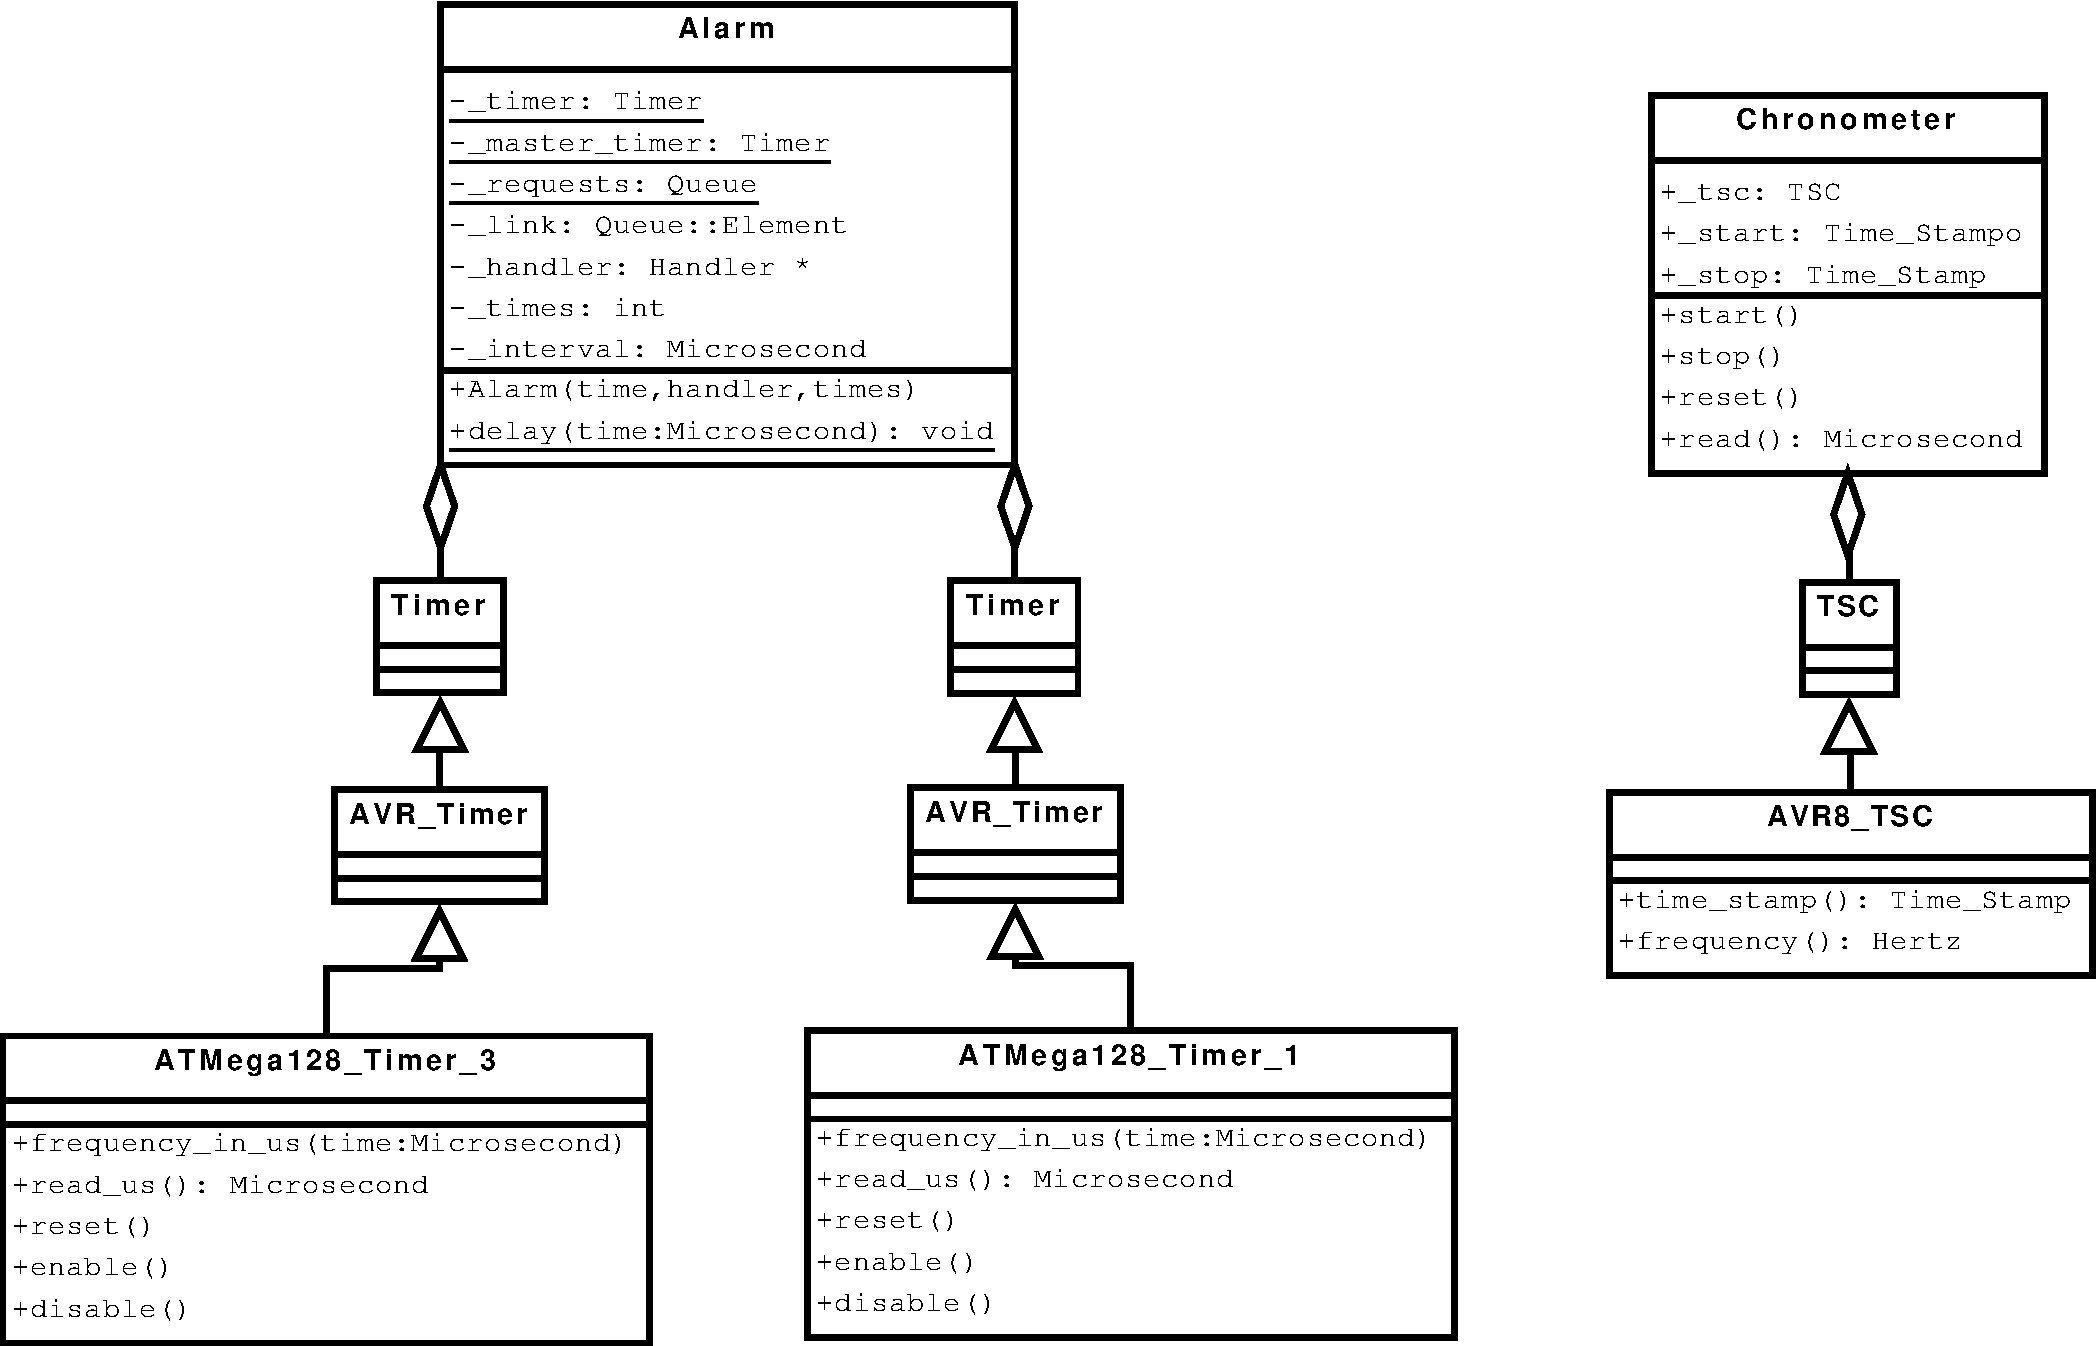
\includegraphics[width=\textwidth]{fig/Alarm_Chronometer_SCCC2008_CR.pdf}
\caption{Classes diagram of EPOS abstractions and hardware mediators (Timers) with one-shot}
\label{fig:alarm_cronometro_classes}
\end{figure*}

In the highest level of \epos{} system, the time is handled by \textit{\textbf{Timepiece}} abstraction family, composed by \textit{\textbf{Clock}}, \textit{\textbf{Alarm}} and \textit{\textbf{Chronometer}} abstractions. Each abstraction has a system specific function. The \textit{\textbf{Clock}} abstraction is responsible to store the current time and is only available in systems that have real-time clock (RTC). The \textit{\textbf{Chronometer}} abstraction is used to perform high precision time measurements and the \textit{\textbf{Alarm}} abstraction can be used to generate events, to wake up a Task/Thread or call a function. This family is supported by \textit{\textbf{Timer}}, \textit{\textbf{TimeStamp Counters (TSC)}} and \textit{\textbf{Real-Time Clocks}} hardware mediators~\cite{marcondes:2006}.

The system periodicity is characterized in the \textit{\textbf{Alarm}} abstraction, that is supported by \textit{\textbf{Timer}} mediator that configures the hardware timer to generate interrupts in a determined frequency. In the timer handler these \textit{ticks} are counted and a routine to verify and to release the scheduled events is executed. In addition to overhead caused by the periodic interrupt handler, if an event is scheduled in a shorter time or not multiple of system period, the invocation of scheduled task can be delayed by rounding errors due to \textit{ticks} granularity. Figure~\ref{fig:alarm_cronometro_classes} presents the classes diagram of the two main abstractions that compose the EPOS time management in the \textit{AVR} architecture. The \textbf{Alarm} abstraction uses two hardware \textit{Timers} available in \textit{AVR} architecture. One of these \textit{Timers}, \textbf{ATMega128\_Timer\_3}, is used to control the \textbf{Alarm} requests queue, this is a 16 bits \textit{Timer}, which allows the alarms scheduling of approximately 9 seconds with the system Clock in $\sim$ 7.2MHz and \textit{PRESCALE} of 1024 in \textit{Timer} Clock. Another \textit{Timer}, \textbf{ATMega128\_Timer\_1}, generates periodic interrupts that trigger the system schedule, these interrupts only occur when the schedule must execute and their time is configured based on the system \textit{QUANTUM}.

The interrupt handler in the periodic time management, in addition of counting \textit{ticks} and release the scheduled events, also invokes the scheduler time handler (\textit{master\_handler}). This routine decreases the scheduler \textit{ticks} counter and verifies if this counter is shorter or equal to zero (QUANTUM ended), calling the thread reschedule routine when necessary.

\begin{figure*}[ht]
\centering
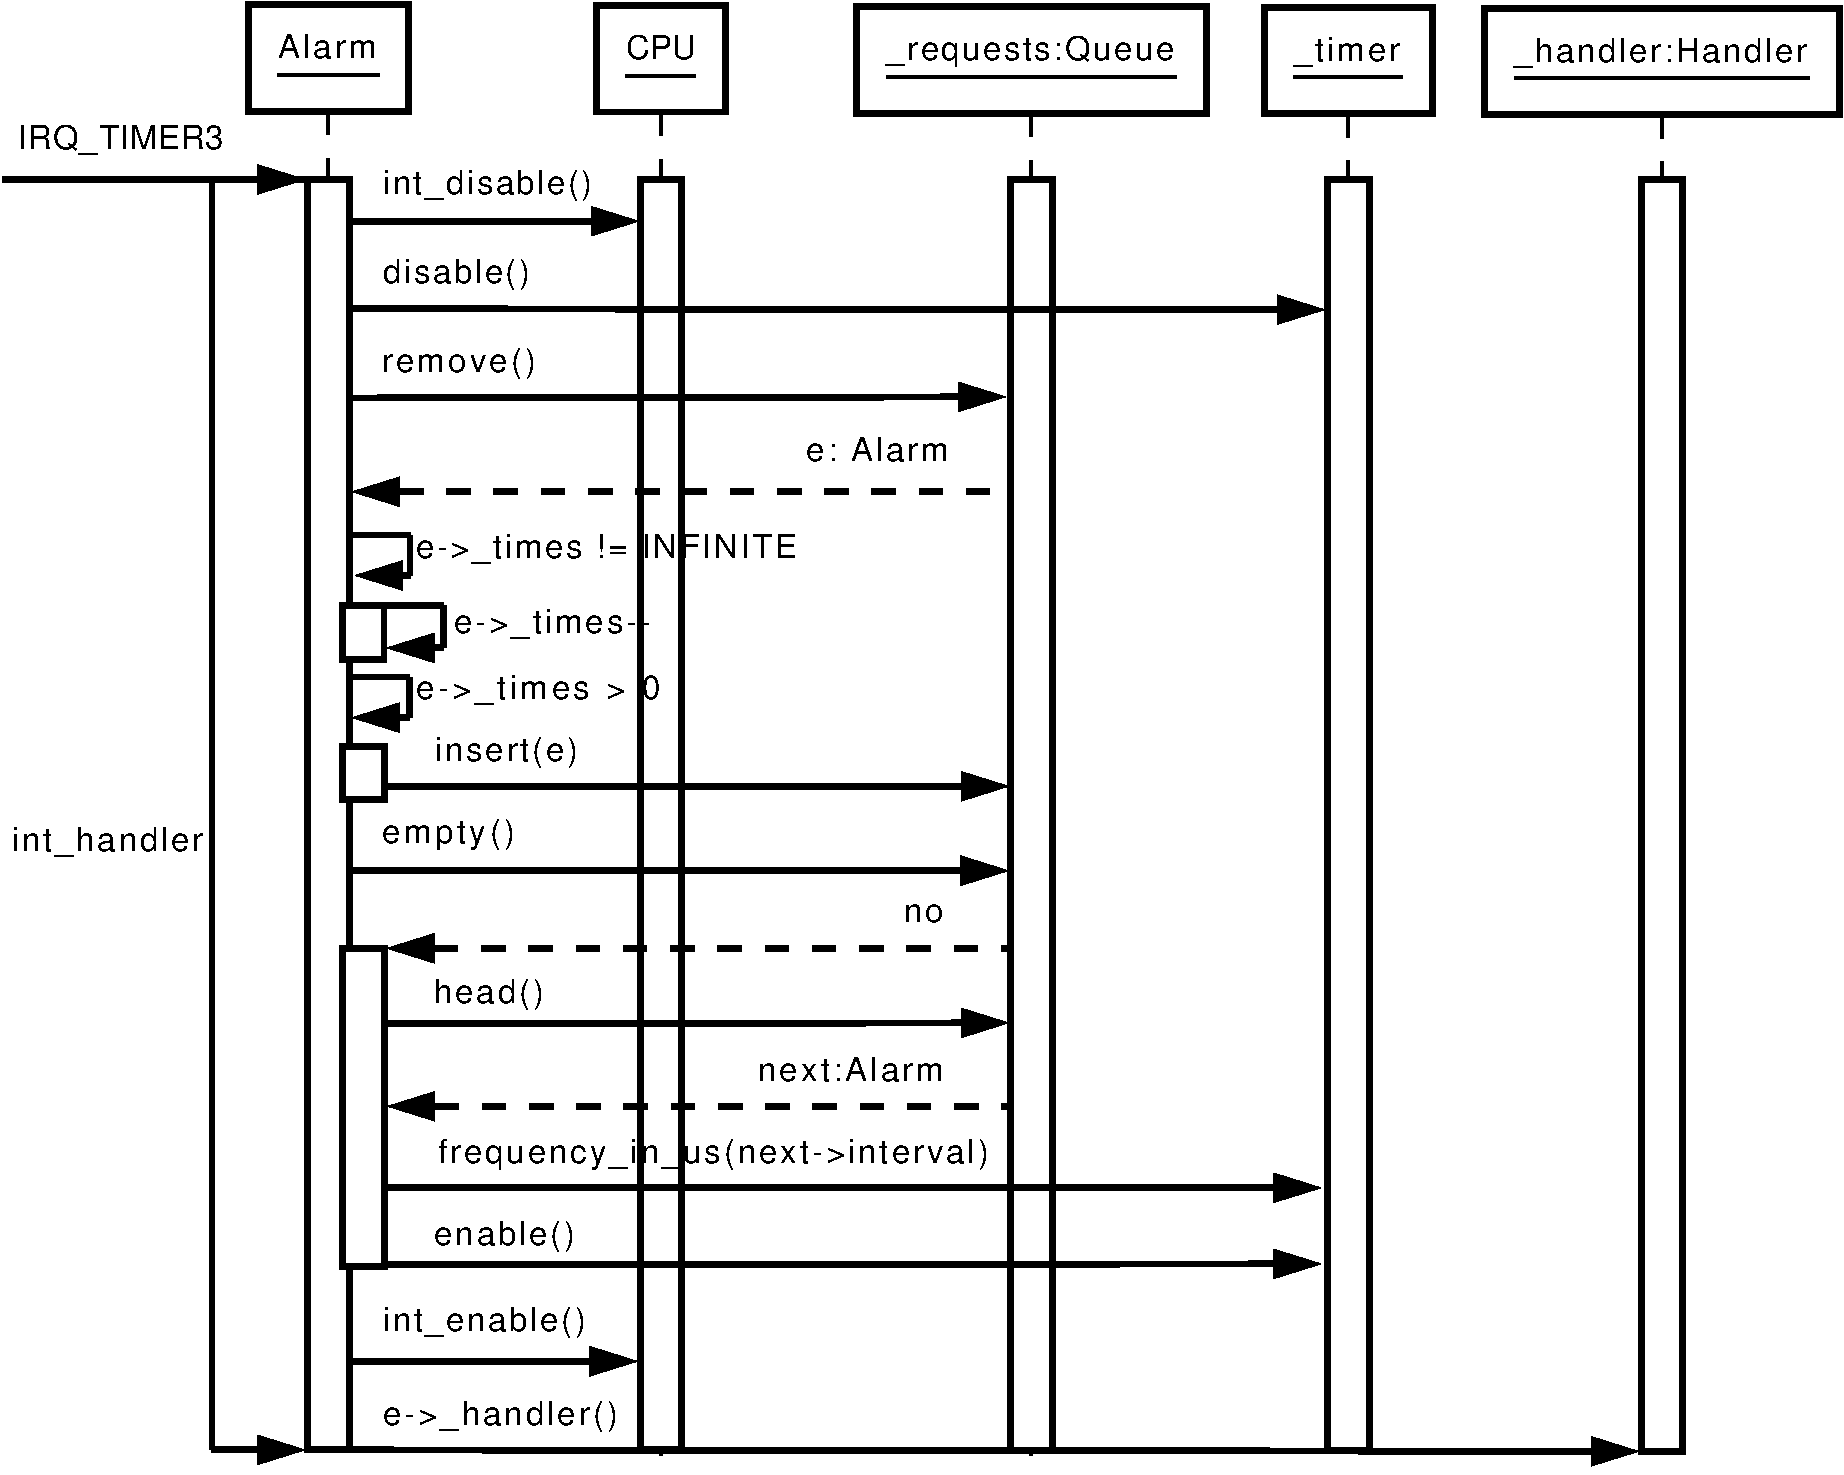
\includegraphics[width=13cm]{fig/int_handler_sequency_SCCC2008_CR.pdf}
\caption{Sequence diagram of EPOS one-shot timer interrupt handler}
\label{fig:ss_timer}
\end{figure*}

The modifications to eliminate the timer periodic interrupts (counting of \textit{ticks}) and to create the timer structure based on one-shot timer focused in the \textbf{Alarm} abstraction. By changing the concept from periodic interrupt to variable interval of the next trigger, the \textit{\textbf{Alarm}} interrupt handler was implemented as the sequence diagram in Figure~\ref{fig:ss_timer}. Unlike of periodic approach, where every \textit{tick} the interrupt handler called \textit{master\_handler}, the new implementation uses two independent hardware timers. One related to alarms requests (\textit{Queue \_requests}), which is programmed to trigger at the precise moment that was scheduled to wake up a task and another timer related to system schedule, programmed to trigger every schedule \textit{QUANTUM}.

In this new implementation, the timer related to scheduling is set in the system initialization and when it is shot simply calls the scheduling routine. This treatment is simple and fast, because it does not need to do the control of the \textit{ticks} number in every interrupt and also decreases the schedule influence in the system. The timer related to alarms only is initialized in the \textbf{Alarm} creation. When it is created, the \textbf{Alarm} is added in an ordered and relative queue, then the added value is exactly the value required to program the timer. When an interrupt arrives, the handler removes the \textbf{Alarm} on the first position in the queue, verifies if there are \textbf{Alarms} in the queue and if exist, reprogram the timer with the next value. This interrupt handler is executed much less than periodic handler, because it is called only when a timer event needs to be handled. We can see the impacts on these numbers in the next section.

%------------------------------------------------------------------------------
\section{Results Analysis}
\label{sec:analise}
To analyze the impact of our One-Shot timer implementation in EPOS was used the well-known Philosophers dinner application \cite{modern}. This implementation of the problem has five threads, that behave like the philosophers, changing their state between thinking and eating. The philosopher needs two forks to eat the Spaghetti and there are five forks on the table, therefore, two non-adjacent philosophers can eat at the same time. The thinking and eating behaviors are a delay (call to the \textbf{Alarm::delay method}) and to eat, the philosopher have to catch two forks that are Semaphores in our implementation (call to \textbf{semaphore.p()}). Each thread executes ten times.

This test application was compiled to Atmel Atmega128 microcontroler. This is an 8 bits microcontroler, with 4KB RAM memory, 128KB flash memory, two 8 bits and one 16 bits timers. As explained in section \ref{sec:gerencia} one 8 bits timer was used to trigger the operating system scheduler and one 16 bits timer was used to manage the Operating System Alarm queue (delays). Four characteristics were analyzed in this tests:

\begin{table*}[t]
\caption{Memory footprint of the test application using both implementations: Periodic and One-Shot Timer}
\centering
%\begin{footnotesize}
\begin{tabular}{|c|c|c|}
\hline
\it Periodic Timer (bytes) & \it Single-shot (bytes) & \it Difference (bytes) \cr
\hline
\textbf{32000} & \textbf{32504} & \textbf{504} \cr
\hline
\end{tabular}
%\end{footnotesize}
\label{tab:mem}
\end{table*}

\begin{table*}[t]
\caption{Number of executions of the interrupt handler. Periodic Time Manager VS Single-Shot Time Manager}
\centering
\begin{tabular}{|c|c|c|c|c|}\hline

\it Scenario & \it Handler 		& \it Periodic 	 & \it Single-Shot   	& \it Difference \cr\hline

Scenario 1 & int\_handler 		& \textbf{26005} & \textbf{100} 	& \textbf{25905}\cr\hline

Scenario 1 & \textit{master\_handler} 	& \textbf{26415} & \textbf{3559} 	& \textbf{22856}\cr\hline

Scenario 2 & int\_handler 		& \textbf{9843}  & \textbf{100} 	& \textbf{9743}	\cr\hline

Scenario 2 & \textit{master\_handler} 	& \textbf{10252} & \textbf{320} 	& \textbf{9932}	\cr\hline

Scenario 3 & int\_handler 		& \textbf{3079}  & \textbf{100} 	& \textbf{2979}	\cr\hline

Scenario 3 & \textit{master\_handler} 	& \textbf{3239}  & \textbf{68} 		& \textbf{3171}	\cr\hline
\end{tabular}
\label{tab:int_handler}
\end{table*}

\begin{enumerate}
\item \textit{Memory footprint}: embedded systems have low resources available, processing, memory and power consumption must be closely adjusted. An embedded operating system must be able to save resources usage. In this context, this metric evaluates the impact of the One-Shot implementation in the final footprint of the system (OS plus application) compared to the traditional implementation with periodic time management.

\item \textit{Threads processing time}: the thread processing time is the amount of time between the thread start time and its finish time. The processing time of a thread may be increased if other thread, with higher priority, is triggered during the thread execution, so the running thread is preempted, and the higher priority thread gets the processor. Therefore, in periodic time management, the running thread is also interfered by the time interrupt handler, as the interrupt handlers have higher priority in the system. In non-periodic time management, the interrupt handler executes only when a thread is ready to execute.

\item \textit{Context switches number}: a context switch happens when a thread that is running is changed for other thread, is possible that the running thread has not finished yet. It is important that when the previous context is restored, the thread resumes by the same execution point it was when preempted.

\item \textit{Interrupt handler execution times}: this characteristic is important to compare how many times the interrupt handler is executed in each implementation. This is an interesting comparison parameter that shows how many times the periodic timer implementation calls the interrupt handler and how many times the One-Shot does, together with the response time, we can examine the trade-off of having a light interrupt handler called many times (periodic timer implementation) VS an interrupt handler that does some computation but is called less times (One-Shot timer).
\end{enumerate}

Table \ref{tab:mem} shows the memory footprint of the two versions of \epos{}, one with periodic time management and other with One-Shot time management. The One-Shot time manager was 504 bytes larger than the periodic time manager. This is expected, as long as the One-Shot time manager uses two different hardware timers, one 8 bits timer to the scheduler and one 16 bits timer to control the Alarm queue, thus two hardware mediators~\cite{Polpeta:2004} were need.

The following tests were done in three scenarios. These scenarios are described bellow, showing the time each philosopher spend thinking and then eating in each execution.
\begin{itemize}
	\item Scenario 1: Thinks for 1000 ms and eats for 5000 ms

	\item Scenario 2: Thinks for 100 ms and eats for 500 ms

	\item Scenario 3: Thinks for 25 ms and eats for 125 ms
\end{itemize}

These Scenarios were tested to analyze the impact of the One-Shot time manager in applications that spend most of their time waiting timer events, as expressed in the following tables and graphs.

Table \ref{tab:int_handler} shows the number of executions of each interrupt handler. Obviously, in the periodic time management, the timer interrupt handler executes every \textit{Tick} ($\sim$ 1,38~ms), even if no timer event exists. Differently, the interrupt timer handler of the One-Shot time manager, only will be executed when there is an event in the queue to be fired, this results in approximately 25905 less executions (Scenario 1). In each \textit{tick}, the periodic time handler calls the \textit{master\_handler} (scheduler), this is the way found to give the scheduler time event the highest priority in the time events, so it runs even if other time event is triggered in the same \textit{tick}. In the One-Shot implementation, the  \textit{master\_handler} will only be triggered when the Scheduler \textit{QUANTUM} is met.

\begin{table}[t]
\caption{Number of Context Switches of the threads (all summed) in the three Scenarios}
\centering
\begin{tabular}{|c|c|c|c|}\hline
\it Scenario 	& \it Periodic & \it Single-shot & \it Difference \cr\hline
Scenario 1 	& \textbf{616} & \textbf{344} 	 & \textbf{272} \cr\hline
Scenario 2 	& \textbf{615} & \textbf{360} 	 & \textbf{255} \cr\hline
Scenario 3 	& \textbf{617} & \textbf{317} 	 & \textbf{300} \cr\hline
\end{tabular}
\label{tab:cs_num}
\end{table}

Table~\ref{tab:cs_num} shows the number of context switches in both versions of \epos{} running the test application. As expected the One-Shot version had up to three hundred less context switches (Scenario 3), this is in someway an effect of less interrupt handler calls, that reduces the effective \textit{QUANTUM} of the \textit{Thread}. Reducing the operating system \textit{overhead}, the time \textit{QUANTUM} to each thread execution is better used, resulting in these preemptions.

\begin{figure}[p]
\centering
\subfigure[Scenario 1]{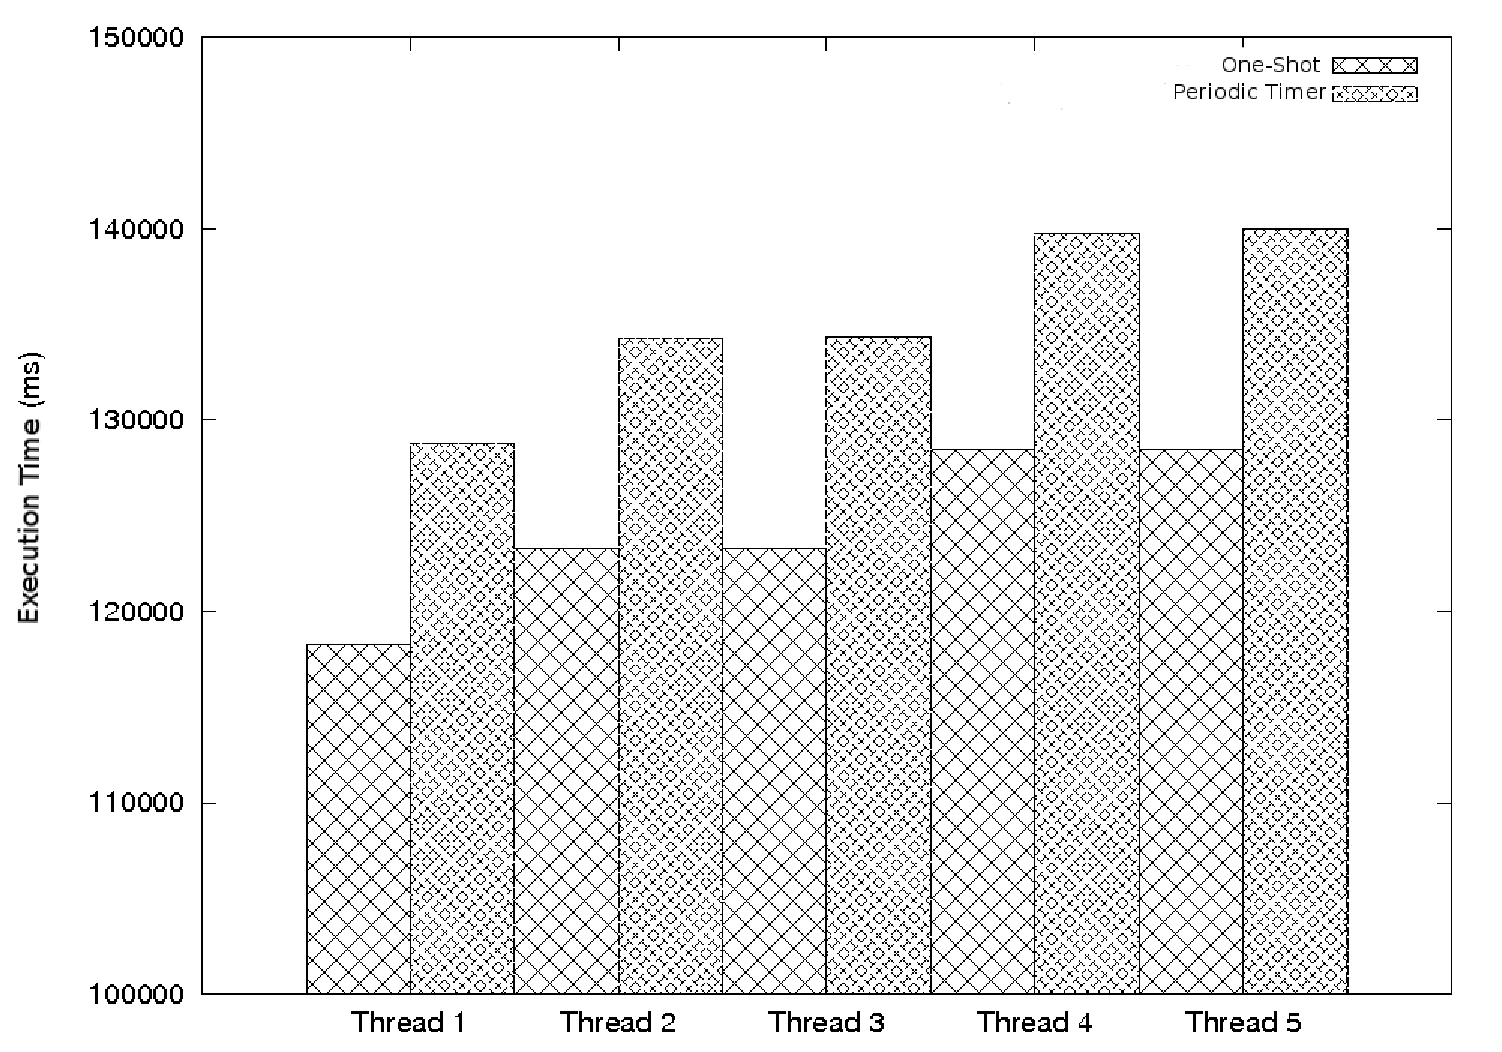
\includegraphics[width=\columnwidth]{fig/cenario1.pdf}}
\subfigure[Scenario 2]{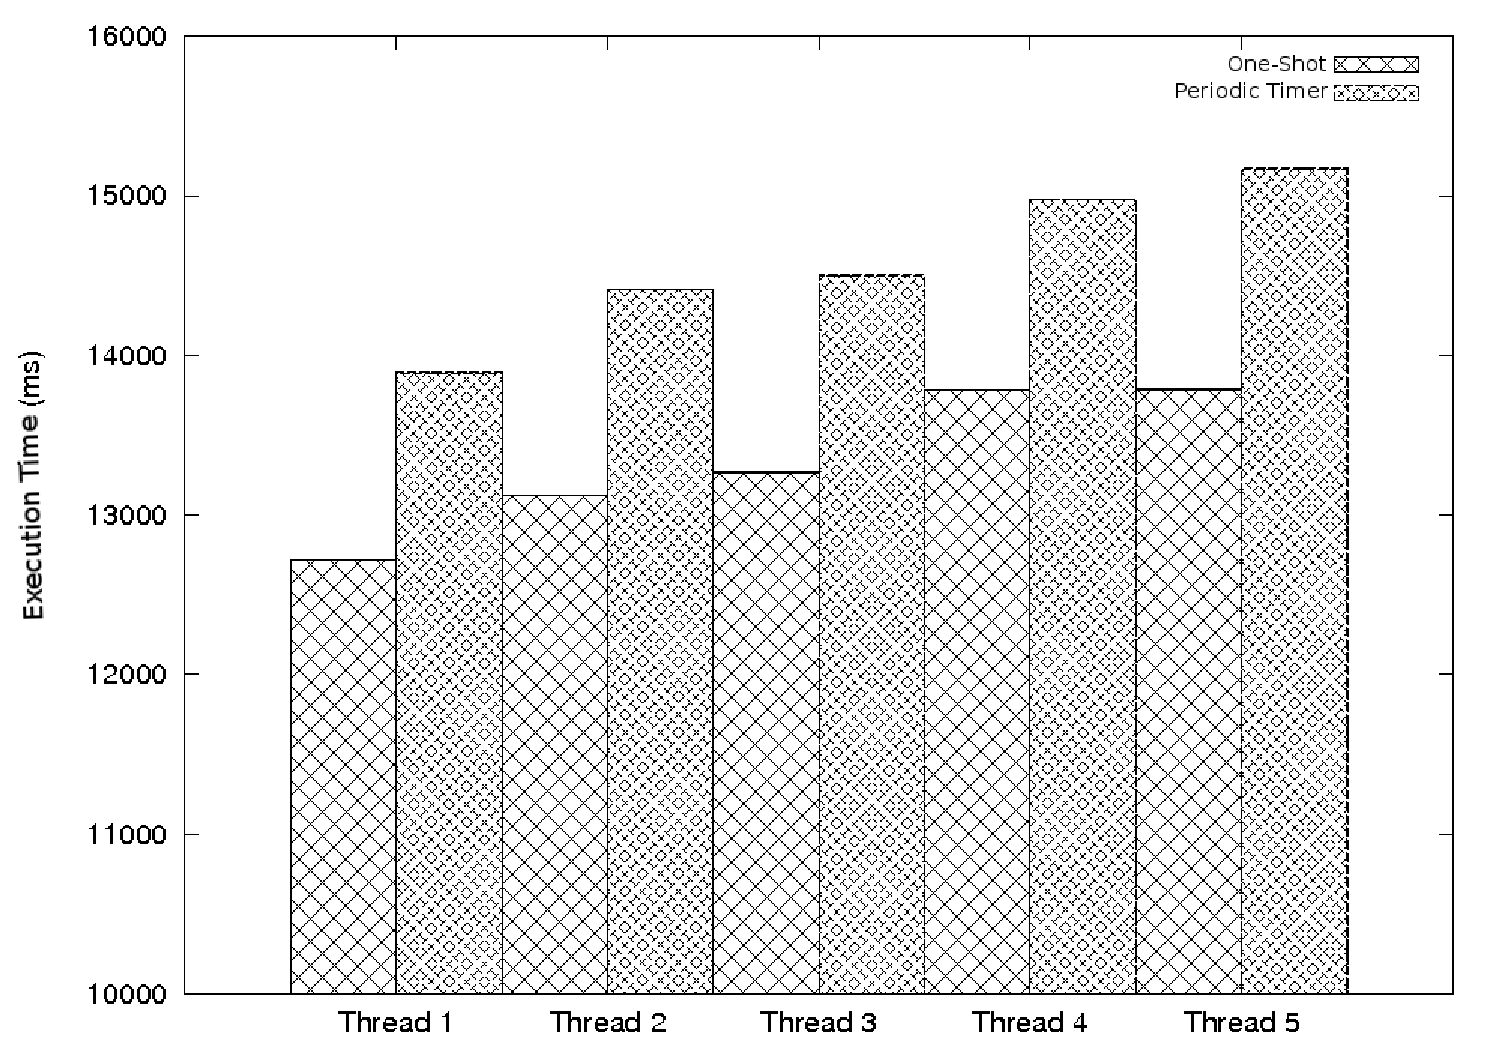
\includegraphics[width=\columnwidth]{fig/cenario2.pdf}}
\subfigure[Scenario 3]{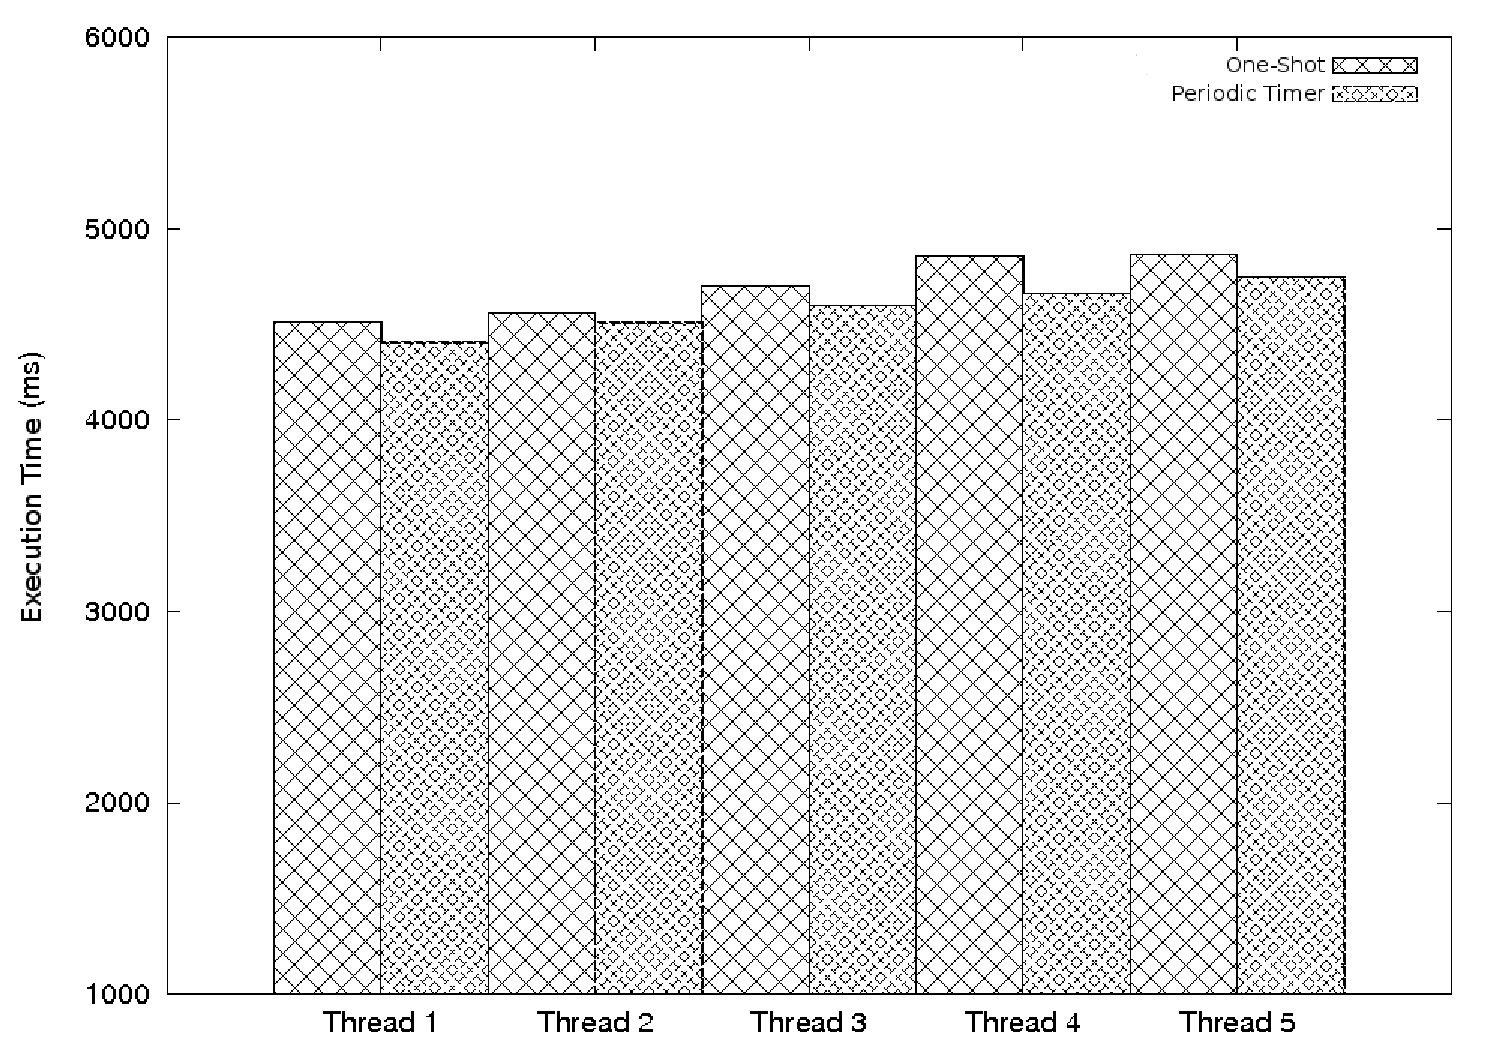
\includegraphics[width=\columnwidth]{fig/cenario3.pdf}}
\caption{Processing time of the threads in the three scenarios}
\label{fig:comp}
\end{figure}

Figure \ref{fig:comp} shows the processing time of the \textit{Threads} (Philosophers) in the three scenarios. Scenarios 1 and 2 shows that the processing time of the threads are smaller in the One-Shot implementation. Scenario 3, where the thinking and eating time of each philosopher (thread) is smaller, is showed that the periodic time manager implementation (\textit{ticks} based) causes less impact in the threads processing time. This happens because the tick size processed by the operating system is quite close to the delay intervals requested by each philosopher (thread), resulting in almost an event triggered in each tick. In conclusion, the processing time would be very similar in both implementations for applications with very small delays times (less than 10000 $\mu$s).

\begin{figure*}[t]
\centering
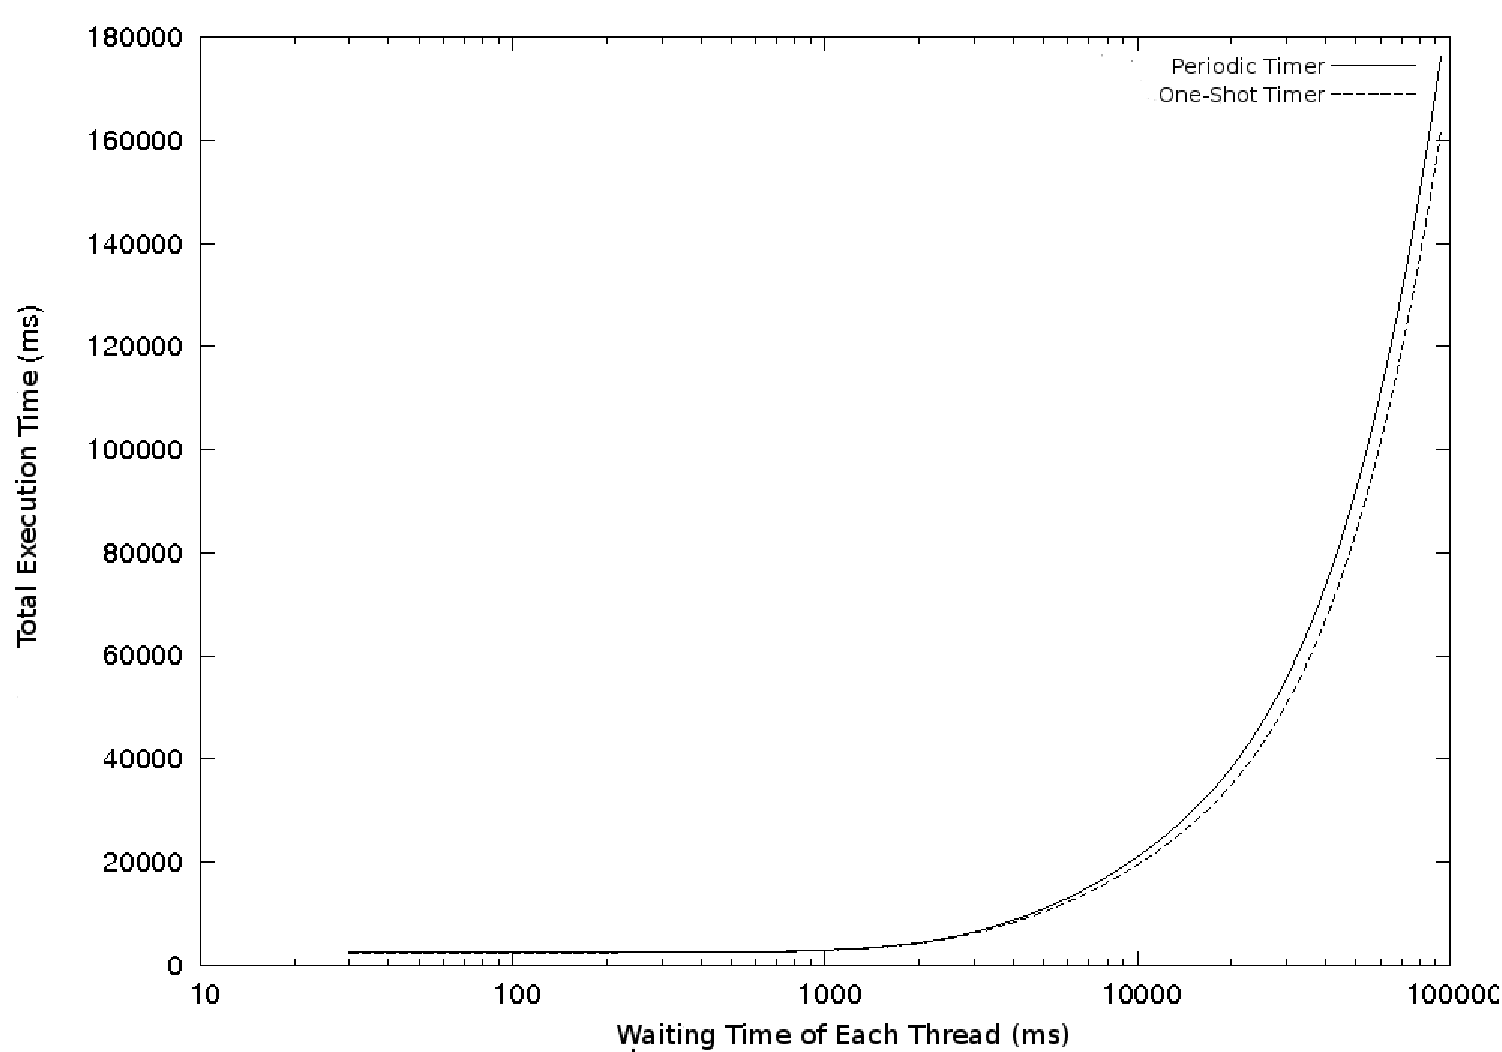
\includegraphics[width=13cm]{fig/sstimer.pdf}
\caption{Total processing time varying the wait time}
\label{fig:curve}
\end{figure*}

Figure \ref{fig:curve} shows a new test series executed in the One-Shot and the periodic implementations varying the delay time (eat and think time) of each thread (philosopher). This figures shows that when the application spends most of the execution time waiting time events, the overhead of the periodic time manager is bigger, resulting in bigger total execution time. in the other hand, when the total waiting time is small, there is little difference in performance of both implementations, resulting in execution times close to each other.

%------------------------------------------------------------------------------
\section{Conclusions and Future Works}
\label{sec:conclusao}

This paper presented a comparison between One-Shot timers and Periodic timers in EPOS time management. Although the one-shot approach is not the most efficient between non-periodic time management algorithms, this implementation has allowed a first view of positive and negative impacts of non-periodic timers class in EPOS.

Four metrics were evaluated in order to measure the impacts of EPOS periodic and non-periodic time management implementations. The number of context switches and the number of interrupt handler executions obtained significant improvements in the system performance. And as expected, the memory consumption of non-periodic implementation was higher, due to use of two timers. The tasks computation time suffer less impact in the One-Shot time management when the application spends most of the time waiting for timer events.

Despite the improve of system performance in the medium case, there are situations where the non-periodic approach can be a bad alternative, for example, when the one-shot timer interrupt handler frequency tends to the frequency of the \textit{ticks} number in the periodic timer. Therefore, the number of handler calls is similar.

The implementation of other more efficient non-periodic time management algorithms, like \textit{smart timers}, is a future work.

\bibliographystyle{latex8}
\bibliography{ss_epos_SCCC2008_CR}

\end{document}